% AI Trip Planner - Design Document (LaTeX Version)
% Compiled for: Development Team
% Date: February 25, 2026
% Version: 1.0

\documentclass[12pt,a4paper]{report}

% Essential Packages
\usepackage[utf8]{inputenc}
\usepackage[T1]{fontenc}
\usepackage[english]{babel}
\usepackage{geometry}
\usepackage{graphicx}
\usepackage{float}
\usepackage{hyperref}
\usepackage{xcolor}
\usepackage{listings}
\usepackage{longtable}
\usepackage{booktabs}
\usepackage{array}
\usepackage{multirow}
\usepackage{enumitem}
\usepackage{fancyhdr}
\usepackage{titlesec}
\usepackage{tocloft}
\usepackage{amsmath}
\usepackage{amssymb}
\usepackage{caption}
\usepackage{subcaption}

% Page Setup
\geometry{
    left=1in,
    right=1in,
    top=1in,
    bottom=1in
}

% Hyperlink Setup
\hypersetup{
    colorlinks=true,
    linkcolor=blue,
    filecolor=magenta,      
    urlcolor=cyan,
    pdftitle={AI Trip Planner - Design Document},
    pdfauthor={Development Team},
    bookmarks=true,
}

% Code Listings Setup
\lstdefinestyle{pythonstyle}{
    language=Python,
    basicstyle=\ttfamily\small,
    keywordstyle=\color{blue},
    commentstyle=\color{green!60!black},
    stringstyle=\color{red},
    numbers=left,
    numberstyle=\tiny\color{gray},
    stepnumber=1,
    numbersep=8pt,
    backgroundcolor=\color{gray!10},
    showspaces=false,
    showstringspaces=false,
    showtabs=false,
    frame=single,
    rulecolor=\color{black},
    tabsize=2,
    breaklines=true,
    breakatwhitespace=false,
    captionpos=b
}

\lstdefinestyle{jsonStyle}{
    basicstyle=\ttfamily\small,
    numbers=left,
    numberstyle=\tiny\color{gray},
    stepnumber=1,
    numbersep=8pt,
    backgroundcolor=\color{gray!10},
    frame=single,
    breaklines=true,
    string=[s]{"}{"},
    stringstyle=\color{blue},
    comment=[l]{:},
    commentstyle=\color{black},
}

\lstdefinestyle{bashStyle}{
    language=bash,
    basicstyle=\ttfamily\small,
    keywordstyle=\color{blue},
    commentstyle=\color{green!60!black},
    numbers=none,
    backgroundcolor=\color{gray!10},
    frame=single,
    breaklines=true,
}

% Header and Footer
\pagestyle{fancy}
\fancyhf{}
\fancyhead[L]{\leftmark}
\fancyhead[R]{AI Trip Planner - Design Document}
\fancyfoot[C]{\thepage}
\renewcommand{\headrulewidth}{0.4pt}
\renewcommand{\footrulewidth}{0.4pt}

% Title Formatting
\titleformat{\chapter}[display]
  {\normalfont\huge\bfseries}{\chaptertitlename\ \thechapter}{20pt}{\Huge}
\titlespacing*{\chapter}{0pt}{-50pt}{40pt}

% Document Information
\title{
    \vspace{2cm}
    \Huge \textbf{Design Document} \\
    \vspace{0.5cm}
    \LARGE AI Trip Planner Agent System \\
    \vspace{2cm}
    \includegraphics[width=0.3\textwidth]{logo.png} \\
    \vspace{2cm}
}

\author{
    \Large Development Team \\
    \vspace{0.5cm}
    \normalsize \texttt{tripplanner@example.com}
}

\date{
    \vspace{1cm}
    \Large Version 1.0 \\
    \vspace{0.3cm}
    \normalsize February 25, 2026 \\
    \vspace{0.3cm}
    \normalsize Status: Final
}

\begin{document}

% Title Page
\maketitle
\thispagestyle{empty}
\newpage

% Document Control Page
\chapter*{Document Control}
\addcontentsline{toc}{chapter}{Document Control}

\begin{table}[H]
\centering
\begin{tabular}{|p{4cm}|p{10cm}|}
\hline
\textbf{Document Title} & Design Document - AI Trip Planner Agent System \\
\hline
\textbf{Version} & 1.0 \\
\hline
\textbf{Date} & February 25, 2026 \\
\hline
\textbf{Status} & Final \\
\hline
\textbf{Classification} & Internal - Technical Documentation \\
\hline
\textbf{Authors} & Development Team \\
\hline
\textbf{Reviewers} & Lead Architect, Backend Lead, Frontend Lead, DevOps Lead, QA Lead \\
\hline
\textbf{Approvers} & Technical Director, CTO \\
\hline
\end{tabular}
\end{table}

\section*{Version History}

\begin{table}[H]
\centering
\begin{tabular}{|c|c|p{6cm}|p{4cm}|}
\hline
\textbf{Version} & \textbf{Date} & \textbf{Changes} & \textbf{Author} \\
\hline
1.0 & 2026-02-25 & Initial design document & Development Team \\
\hline
\end{tabular}
\end{table}

\newpage

% Table of Contents
\tableofcontents
\newpage

% List of Figures
\listoffigures
\newpage

% List of Tables
\listoftables
\newpage

%========================================
% CHAPTER 1: INTRODUCTION
%========================================
\chapter{Introduction}

\section{Purpose}

This design document provides a comprehensive technical blueprint for the AI Trip Planner Agent system. It describes the architecture, components, interfaces, data structures, and design decisions that guide the implementation of this intelligent travel itinerary generation system.

\subsection{Target Audience}

\begin{itemize}
    \item Software architects and senior developers
    \item Backend and frontend development teams
    \item DevOps and infrastructure engineers
    \item Technical leads and system integrators
    \item Quality assurance and testing teams
\end{itemize}

\section{Scope}

This document covers the complete technical design of an AI-powered trip planning system that leverages LangChain agents with the ReAct (Reasoning + Acting) pattern to generate personalized travel itineraries.

\subsection{System Capabilities}

\begin{itemize}
    \item AI agent orchestration using LangChain framework
    \item Integration with external APIs (Groq, OpenStreetMap, Open-Meteo, Overpass, OpenRouteService)
    \item Real-time data aggregation and processing
    \item Structured itinerary generation with budget tracking
    \item Responsive web interface with modern UX
    \item RESTful API with FastAPI framework
\end{itemize}

\subsection{Technology Stack}

\begin{itemize}
    \item \textbf{Backend:} Python 3.9+, FastAPI, LangChain, Pydantic
    \item \textbf{Frontend:} HTML5, CSS3, JavaScript (ES6+)
    \item \textbf{AI/LLM:} Groq API with Llama 3.1 models
    \item \textbf{External APIs:} OpenStreetMap, Open-Meteo, Overpass API, OpenRouteService
    \item \textbf{Deployment:} Docker, Cloud platforms (AWS/Azure/GCP)
\end{itemize}

\section{Definitions and Acronyms}

\begin{table}[H]
\centering
\begin{tabular}{|p{3cm}|p{11cm}|}
\hline
\textbf{Term} & \textbf{Definition} \\
\hline
Agent & Autonomous AI system that reasons and uses tools \\
\hline
ReAct & Reasoning + Acting pattern for AI agents \\
\hline
LangChain & Framework for building LLM-powered applications \\
\hline
Groq & Ultra-fast AI inference platform \\
\hline
POI & Point of Interest (tourist attractions, restaurants, etc.) \\
\hline
Nominatim & OpenStreetMap's geocoding service \\
\hline
Overpass & OpenStreetMap's query API for POI data \\
\hline
FastAPI & Modern Python web framework for building APIs \\
\hline
Pydantic & Data validation library using Python type hints \\
\hline
CORS & Cross-Origin Resource Sharing \\
\hline
LLM & Large Language Model \\
\hline
REST & Representational State Transfer \\
\hline
\end{tabular}
\caption{Definitions and Acronyms}
\label{tab:definitions}
\end{table}

\section{Design Goals}

\begin{enumerate}
    \item \textbf{Performance:} Generate complete itineraries in under 60 seconds
    \item \textbf{Scalability:} Support concurrent users without performance degradation
    \item \textbf{Reliability:} Graceful handling of external API failures with fallbacks
    \item \textbf{Maintainability:} Modular architecture with clear separation of concerns
    \item \textbf{Usability:} Intuitive interface with real-time feedback
    \item \textbf{Security:} Secure API key management and input validation
    \item \textbf{Extensibility:} Easy addition of new tools and features
\end{enumerate}

\section{References}

\begin{itemize}
    \item Software Requirements Specification (SRS-Document.md)
    \item Architecture Documentation (ARCHITECTURE.md)
    \item API Documentation (FastAPI /docs endpoint)
    \item LangChain Documentation: \url{https://python.langchain.com/}
    \item Groq API Docs: \url{https://console.groq.com/docs}
    \item FastAPI Documentation: \url{https://fastapi.tiangolo.com/}
\end{itemize}

%========================================
% CHAPTER 2: SYSTEM OVERVIEW
%========================================
\chapter{System Overview}

\section{System Context}

The AI Trip Planner is a standalone web-based application that integrates with multiple external services to provide intelligent travel planning capabilities. The system acts as an intermediary between users and various data sources, leveraging AI to synthesize information into coherent travel itineraries.

\begin{figure}[H]
    \centering
    \includegraphics[width=0.9\textwidth]{system-context-diagram.png}
    \caption{System Context Diagram}
    \label{fig:system-context}
\end{figure}

\section{High-Level Architecture}

The system follows a three-tier architecture:

\begin{enumerate}
    \item \textbf{Presentation Layer (Frontend)}
    \begin{itemize}
        \item Single-page web application
        \item Responsive UI for desktop and mobile
        \item Client-side validation and state management
    \end{itemize}
    
    \item \textbf{Application Layer (Backend)}
    \begin{itemize}
        \item FastAPI REST API server
        \item AI agent orchestration with LangChain
        \item Business logic and data processing
        \item External API integration
    \end{itemize}
    
    \item \textbf{Data Layer (External Services)}
    \begin{itemize}
        \item Groq API for LLM inference
        \item OpenStreetMap for geocoding and POI data
        \item Open-Meteo for weather forecasts
        \item OpenRouteService for route optimization
    \end{itemize}
\end{enumerate}

\begin{figure}[H]
    \centering
    \includegraphics[width=0.9\textwidth]{high-level-architecture-diagram.png}
    \caption{High-Level Architecture Diagram}
    \label{fig:high-level-arch}
\end{figure}

\section{Key Design Patterns}

\subsection{ReAct Agent Pattern}

The core of the system uses the ReAct (Reasoning + Acting) pattern for AI agents:

\begin{lstlisting}[style=bashStyle]
Thought: Analyze what information is needed
Action: Call a tool to gather data
Observation: Process tool output
... (repeat as needed)
Final Answer: Synthesize structured itinerary
\end{lstlisting}

\subsection{Service Layer Pattern}

Business logic is separated into service layers:
\begin{itemize}
    \item \texttt{trip\_service.py}: Orchestrates trip planning workflow
    \item \texttt{api\_service.py}: Manages external API calls
    \item Clear separation between routes (controllers) and services
\end{itemize}

\subsection{Repository Pattern}

External API calls are abstracted through a service layer, making it easy to:
\begin{itemize}
    \item Mock services for testing
    \item Add caching layers
    \item Implement retry logic
    \item Switch API providers
\end{itemize}

\subsection{Strategy Pattern}

The system uses strategy pattern for different trip planning approaches:
\begin{itemize}
    \item Fast mode (direct API calls with LLM formatting)
    \item Agent mode (ReAct pattern with tool usage)
    \item Configurable via settings or request parameters
\end{itemize}

%========================================
% CHAPTER 3: SYSTEM ARCHITECTURE
%========================================
\chapter{System Architecture}

\section{Architectural Style}

The system implements a \textbf{Layered Architecture} with \textbf{Microservices principles}:

\begin{itemize}
    \item \textbf{Separation of Concerns:} Frontend, backend, and external services are clearly separated
    \item \textbf{Stateless Design:} No server-side session management
    \item \textbf{API-First:} RESTful API as the primary interface
    \item \textbf{Cloud-Native:} Containerized for easy deployment
\end{itemize}

\section{Component Architecture}

\begin{figure}[H]
    \centering
    \includegraphics[width=0.95\textwidth]{component-architecture-diagram.png}
    \caption{Complete Component Architecture}
    \label{fig:component-arch}
\end{figure}

\subsection{Frontend Components}

\subsubsection{index.html}
\begin{itemize}
    \item Trip planning form
    \item Loading state UI
    \item Results display area
    \item Error handling UI
\end{itemize}

\subsubsection{app.js}
\begin{itemize}
    \item Form submission handler
    \item State management (currentTrip, isLoading)
    \item UI controller (showSection, displayResults)
    \item Loading animation controller
    \item PDF generation
\end{itemize}

\subsubsection{api.js}
\begin{itemize}
    \item HTTP client wrapper
    \item API endpoint calls
    \item Error handling
    \item Request/response transformation
\end{itemize}

\subsubsection{styles.css}
\begin{itemize}
    \item Professional design system
    \item Responsive layouts
    \item Component styling
    \item Animations and transitions
\end{itemize}

\subsection{Backend Components}

\subsubsection{main.py}
\begin{itemize}
    \item FastAPI application initialization
    \item CORS configuration
    \item Route registration
    \item Global exception handling
    \item Startup/shutdown events
\end{itemize}

\subsubsection{routes/trip\_planner.py}
\begin{itemize}
    \item \texttt{/api/plan-trip} endpoint
    \item \texttt{/api/health} endpoint
    \item Request validation
    \item Response formatting
\end{itemize}

\subsubsection{services/trip\_service.py}
\begin{itemize}
    \item \texttt{plan\_trip()}: Main orchestration method
    \item \texttt{plan\_trip\_fast()}: Fast mode implementation
    \item Response formatting
    \item Business logic coordination
\end{itemize}

\subsubsection{services/api\_service.py}
\begin{itemize}
    \item \texttt{get\_coordinates()}: Geocoding via Nominatim
    \item \texttt{get\_weather\_forecast()}: Weather data via Open-Meteo
    \item \texttt{get\_points\_of\_interest()}: POI search via Overpass
    \item \texttt{get\_route\_info()}: Route calculation via OpenRouteService
    \item HTTP client management
    \item Error handling and retries
\end{itemize}

\subsubsection{agents/trip\_agent.py}
\begin{itemize}
    \item LangChain agent initialization
    \item ReAct pattern implementation
    \item Tool registration and management
    \item Agent prompt engineering
    \item Response parsing
\end{itemize}

\subsubsection{agents/tools.py}
\begin{itemize}
    \item Tool definitions for LangChain
    \item Input/output schemas
    \item Tool execution logic
    \item Async-to-sync wrappers
\end{itemize}

\subsubsection{models/schemas.py}
\begin{itemize}
    \item Pydantic models for validation
    \item Request schemas (TripRequest)
    \item Response schemas (TripResponse, DayItinerary, Activity)
    \item Validation rules
\end{itemize}

\subsubsection{utils/config.py}
\begin{itemize}
    \item Environment variable management
    \item Settings class with defaults
    \item API endpoint configuration
    \item Feature flags
\end{itemize}

\subsubsection{utils/helpers.py}
\begin{itemize}
    \item Date calculations
    \item Budget allocation
    \item Distance calculations (Haversine)
    \item Common utilities
\end{itemize}

\section{Data Flow Architecture}

\begin{figure}[H]
    \centering
    \includegraphics[width=0.95\textwidth]{data-flow-diagram.png}
    \caption{Request/Response Data Flow}
    \label{fig:data-flow}
\end{figure}

\subsection{Flow Description}

\begin{enumerate}
    \item \textbf{User Input (Frontend)} - User fills trip planning form, client-side validation, form data serialization
    \item \textbf{API Request (Frontend → Backend)} - POST request to \texttt{/api/plan-trip}, JSON payload with trip parameters
    \item \textbf{Request Processing (Backend)} - FastAPI receives and validates request, Pydantic model validation
    \item \textbf{Trip Planning Orchestration} - Calculate trip metrics (duration, daily budget), parallel external API calls
    \item \textbf{External Data Collection} - Geocoding, weather forecast, points of interest, route information
    \item \textbf{AI Agent Processing} - LangChain agent initialized, ReAct pattern execution, tool calls for data gathering
    \item \textbf{Response Generation} - Format daily itineraries, calculate costs and timings, generate recommendations
    \item \textbf{API Response (Backend → Frontend)} - JSON response with complete itinerary
    \item \textbf{Results Display (Frontend)} - Parse JSON response, render UI components, display itinerary cards
\end{enumerate}

\section{Deployment Architecture}

\begin{figure}[H]
    \centering
    \includegraphics[width=0.95\textwidth]{deployment-architecture-diagram.png}
    \caption{Deployment Architecture}
    \label{fig:deployment-arch}
\end{figure}

\subsection{Components}

\begin{enumerate}
    \item \textbf{Client Browser} - HTML/CSS/JS files, state management, API communication
    \item \textbf{Application Server} - Docker container with Python 3.9+, FastAPI with Uvicorn ASGI server, 2GB+ RAM, 2+ CPU cores
    \item \textbf{External Services} - Groq API, OpenStreetMap services, Open-Meteo, OpenRouteService (all HTTPS)
    \item \textbf{Cloud Platform} - Load balancer, auto-scaling groups, CDN for static files, monitoring and logging
\end{enumerate}

%========================================
% CHAPTER 4: DATA DESIGN
%========================================
\chapter{Data Design}

\section{Data Models}

\begin{figure}[H]
    \centering
    \includegraphics[width=0.9\textwidth]{data-models-diagram.png}
    \caption{Data Models and Relationships}
    \label{fig:data-models}
\end{figure}

\section{Request Schemas}

\subsection{TripRequest}

\begin{lstlisting}[style=pythonstyle, caption={TripRequest Schema}]
class TripRequest(BaseModel):
    destination: str       # City or location name (min 2 chars)
    start_date: str       # YYYY-MM-DD format
    end_date: str         # YYYY-MM-DD format
    budget: float         # Total budget in USD (>= 100)
    travelers: int        # Number of travelers (1-20)
    interests: List[str]  # e.g., ["culture", "food", "museums"]
    pace: str            # "relaxed", "balanced", or "packed"
\end{lstlisting}

\subsubsection{Validation Rules}
\begin{itemize}
    \item \texttt{start\_date} must be $\geq$ today
    \item \texttt{end\_date} must be $>$ \texttt{start\_date}
    \item Trip duration: 1-14 days
    \item \texttt{budget} $\geq$ 100
    \item \texttt{travelers} between 1 and 20
    \item \texttt{pace} must be in allowed values
\end{itemize}

\subsubsection{Example Request}

\begin{lstlisting}[style=jsonStyle, caption={Example Trip Request}]
{
  "destination": "Paris, France",
  "start_date": "2026-06-15",
  "end_date": "2026-06-18",
  "budget": 1500.0,
  "travelers": 2,
  "interests": ["culture", "food", "museums", "architecture"],
  "pace": "balanced"
}
\end{lstlisting}

\section{Response Schemas}

\subsection{TripResponse}

\begin{lstlisting}[style=pythonstyle, caption={TripResponse Schema}]
class TripResponse(BaseModel):
    overview: TripOverview               # Trip summary
    itinerary: List[DayItinerary]       # Daily plans
    smart_additions: SmartAdditions     # Recommendations
\end{lstlisting}

\subsection{TripOverview}

\begin{lstlisting}[style=pythonstyle, caption={TripOverview Schema}]
class TripOverview(BaseModel):
    destination: str                    # Full destination name
    duration: int                       # Number of days
    start_date: str                     # YYYY-MM-DD
    end_date: str                       # YYYY-MM-DD
    total_budget: float                 # Total budget
    daily_budget: float                 # Budget per day
    travelers: int                      # Number of travelers
    weather_summary: str                # Overall weather description
    coordinates: Dict[str, float]       # {"lat": 48.8566, "lon": 2.3522}
\end{lstlisting}

\subsection{DayItinerary}

\begin{lstlisting}[style=pythonstyle, caption={DayItinerary Schema}]
class DayItinerary(BaseModel):
    day: int                    # Day number (1, 2, 3...)
    date: str                   # YYYY-MM-DD
    morning: Activity           # Morning activity
    afternoon: Activity         # Afternoon activity
    evening: Activity           # Evening activity
    weather: str                # Weather description
    travel_time: str            # Estimated travel time
    total_cost: float           # Total cost for the day
    notes: Optional[str]        # Additional notes
\end{lstlisting}

\subsection{Activity}

\begin{lstlisting}[style=pythonstyle, caption={Activity Schema}]
class Activity(BaseModel):
    name: str                   # Activity name
    description: str            # Detailed description
    duration: str               # e.g., "2 hours"
    estimated_cost: float       # Cost in USD
    location: Optional[str]     # Location name
    time_of_day: str           # "morning", "afternoon", or "evening"
\end{lstlisting}

\subsection{SmartAdditions}

\begin{lstlisting}[style=pythonstyle, caption={SmartAdditions Schema}]
class SmartAdditions(BaseModel):
    packing_list: List[str]           # Weather-appropriate items
    weather_tips: List[str]           # Weather-based advice
    alternate_activities: List[str]   # Backup options
    local_tips: List[str]             # Cultural insights
\end{lstlisting}

\section{External API Data Models}

\subsection{Geocoding Data (Nominatim)}

\begin{lstlisting}[style=jsonStyle, caption={Nominatim API Response}]
{
    "lat": 48.8566,                 # Latitude
    "lon": 2.3522,                  # Longitude
    "display_name": "Paris, France", # Full formatted address
    "importance": 0.878             # Relevance score
}
\end{lstlisting}

\subsection{Weather Data (Open-Meteo)}

\begin{lstlisting}[style=jsonStyle, caption={Open-Meteo API Response}]
{
    "daily": {
        "time": ["2026-06-15", "2026-06-16", "2026-06-17"],
        "temperature_2m_max": [23.4, 24.1, 22.8],
        "temperature_2m_min": [15.2, 16.0, 15.8],
        "precipitation_sum": [0.0, 0.0, 2.3],
        "weathercode": [0, 1, 3]
    }
}
\end{lstlisting}

\subsection{POI Data (Overpass)}

\begin{lstlisting}[style=jsonStyle, caption={Overpass API Response}]
{
    "elements": [{
        "type": "node",
        "id": 123456,
        "lat": 48.8584,
        "lon": 2.2945,
        "tags": {
            "name": "Eiffel Tower",
            "tourism": "attraction"
        }
    }]
}
\end{lstlisting}

\section{Database Design}

\textbf{Note:} Current version does not use a persistent database. The system is stateless.

\subsection{Future Enhancements}

\begin{itemize}
    \item User accounts and saved trips (PostgreSQL/MongoDB)
    \item Trip history and favorites
    \item Caching layer (Redis)
    \item Analytics data
\end{itemize}

\begin{figure}[H]
    \centering
    \includegraphics[width=0.95\textwidth]{er-diagram-future.png}
    \caption{Entity-Relationship Diagram (Future Enhancement)}
    \label{fig:er-diagram}
\end{figure}

%========================================
% CHAPTER 5: COMPONENT DESIGN
%========================================
\chapter{Component Design}

\section{Frontend Components}

\subsection{Form Component}

\textbf{Purpose:} Collect user input for trip planning

\textbf{Responsibilities:}
\begin{itemize}
    \item Render input fields
    \item Client-side validation
    \item Form submission handling
    \item Error display
\end{itemize}

\textbf{Key Methods:}
\begin{lstlisting}[language=JavaScript, style=pythonstyle, caption={Form Component Methods}]
function validateFormData(formData) {
    // Validate required fields
    // Check date logic
    // Verify budget minimum
    // Return true/false
}

function getFormData() {
    // Extract form values
    // Parse interests array
    // Return formatted object
}

function handleFormSubmit(event) {
    // Prevent default
    // Validate data
    // Call API
    // Handle response/errors
}
\end{lstlisting}

\subsection{Loading Component}

\textbf{Purpose:} Provide visual feedback during processing

\textbf{Responsibilities:}
\begin{itemize}
    \item Display loading spinner
    \item Show progress bar
    \item Animate loading steps
    \item Display status messages
\end{itemize}

\subsection{Results Component}

\textbf{Purpose:} Display generated itinerary

\textbf{Responsibilities:}
\begin{itemize}
    \item Render trip overview
    \item Display daily itineraries
    \item Show recommendations
    \item Enable download/print
\end{itemize}

\section{Backend Components}

\subsection{Route Handler}

\begin{lstlisting}[style=pythonstyle, caption={API Endpoints}]
@router.post("/api/plan-trip", response_model=TripResponse)
async def plan_trip(request: TripRequest):
    # Validate Groq API key
    # Call trip_service.plan_trip()
    # Return TripResponse
    # Handle exceptions
    pass

@router.get("/api/health")
async def health_check():
    # Return service health status
    pass
\end{lstlisting}

\subsection{Trip Service}

\begin{lstlisting}[style=pythonstyle, caption={Trip Service Methods}]
class TripService:
    async def plan_trip(self, request: TripRequest) -> TripResponse:
        # Main orchestration method
        pass
    
    async def plan_trip_fast(self, request: TripRequest) -> Dict:
        # Fast mode implementation
        # Parallel API calls
        # LLM-based formatting
        pass
\end{lstlisting}

\subsection{API Service}

\begin{lstlisting}[style=pythonstyle, caption={API Service Methods}]
class APIService:
    async def get_coordinates(self, location: str):
        # Call Nominatim API
        pass
    
    async def get_weather_forecast(self, lat, lon, start, end):
        # Call Open-Meteo API
        pass
    
    async def get_points_of_interest(self, lat, lon, radius):
        # Call Overpass API
        pass
\end{lstlisting}

%========================================
% CHAPTER 6: INTERFACE DESIGN
%========================================
\chapter{Interface Design}

\section{User Interface Design}

\subsection{Design Principles}

\begin{itemize}
    \item \textbf{Simplicity:} Clean, uncluttered interface
    \item \textbf{Responsiveness:} Mobile-first design, works on all screen sizes
    \item \textbf{Feedback:} Real-time validation and loading states
    \item \textbf{Accessibility:} WCAG 2.1 Level AA compliance
    \item \textbf{Consistency:} Uniform styling and interaction patterns
\end{itemize}

\begin{figure}[H]
    \centering
    \includegraphics[width=0.85\textwidth]{ui-mockup.png}
    \caption{User Interface Mockup}
    \label{fig:ui-mockup}
\end{figure}

\subsection{Form Design}

\begin{table}[H]
\centering
\begin{tabular}{|l|l|p{4cm}|p{4cm}|}
\hline
\textbf{Field} & \textbf{Type} & \textbf{Validation} & \textbf{Placeholder} \\
\hline
Destination & Text & Required, min 2 chars & "e.g., Paris, France" \\
\hline
Start Date & Date & Required, $\geq$ today & YYYY-MM-DD \\
\hline
End Date & Date & Required, $>$ start\_date & YYYY-MM-DD \\
\hline
Budget & Number & Required, $\geq$ 100 & "e.g., 1500" \\
\hline
Travelers & Number & 1-20 & "2" \\
\hline
Interests & Checkboxes & At least 1 selected & Multiple options \\
\hline
Pace & Radio & One required & relaxed/balanced/packed \\
\hline
\end{tabular}
\caption{Form Field Specifications}
\label{tab:form-fields}
\end{table}

\section{API Interface Design}

\subsection{REST API Endpoints}

\begin{table}[H]
\centering
\begin{tabular}{|l|l|p{5cm}|l|}
\hline
\textbf{Endpoint} & \textbf{Method} & \textbf{Purpose} & \textbf{Auth} \\
\hline
\texttt{/api/plan-trip} & POST & Generate trip itinerary & None \\
\hline
\texttt{/api/health} & GET & Health check & None \\
\hline
\texttt{/api/sample-request} & GET & Get example request & None \\
\hline
\texttt{/docs} & GET & Interactive API docs & None \\
\hline
\texttt{/redoc} & GET & Alternative API docs & None \\
\hline
\end{tabular}
\caption{API Endpoint Summary}
\label{tab:api-endpoints}
\end{table}

\subsection{HTTP Status Codes}

\begin{table}[H]
\centering
\begin{tabular}{|c|l|p{8cm}|}
\hline
\textbf{Code} & \textbf{Meaning} & \textbf{Usage} \\
\hline
200 & OK & Successful trip planning \\
\hline
400 & Bad Request & Invalid input data \\
\hline
422 & Unprocessable Entity & Pydantic validation error \\
\hline
500 & Internal Server Error & Server-side error \\
\hline
503 & Service Unavailable & External API failure \\
\hline
\end{tabular}
\caption{HTTP Status Codes}
\label{tab:http-codes}
\end{table}

%========================================
% CHAPTER 7: API DESIGN
%========================================
\chapter{API Design}

\section{RESTful API Principles}

The API follows REST architectural constraints:

\begin{enumerate}
    \item \textbf{Client-Server:} Clear separation between frontend and backend
    \item \textbf{Stateless:} No server-side session management
    \item \textbf{Cacheable:} Responses include cache control headers
    \item \textbf{Uniform Interface:} Consistent URI structure and HTTP methods
    \item \textbf{Layered System:} Can add caching/load balancing layers
\end{enumerate}

\section{API Versioning Strategy}

\textbf{Current:} No versioning (v1 implicit)

\textbf{Future Strategy:}
\begin{itemize}
    \item URL versioning: \texttt{/api/v1/plan-trip}, \texttt{/api/v2/plan-trip}
    \item Header versioning: \texttt{Accept: application/vnd.tripplanner.v1+json}
    \item Maintain backward compatibility for at least 2 versions
\end{itemize}

\section{Request/Response Patterns}

\subsection{Standard Success Response}

\begin{lstlisting}[style=jsonStyle, caption={Success Response Format}]
{
  "status": "success",
  "data": {...},
  "metadata": {
    "timestamp": "2026-02-25T10:30:00Z",
    "duration_ms": 4532
  }
}
\end{lstlisting}

\subsection{Standard Error Response}

\begin{lstlisting}[style=jsonStyle, caption={Error Response Format}]
{
  "status": "error",
  "message": "Human-readable error message",
  "code": "ERROR_CODE",
  "detail": "Technical details",
  "timestamp": "2026-02-25T10:30:00Z"
}
\end{lstlisting}

\section{API Security}

\subsection{CORS Configuration}

\begin{lstlisting}[style=pythonstyle, caption={CORS Settings}]
allow_origins = [
    "http://localhost:3000",
    "http://localhost:8000"
]
allow_methods = ["GET", "POST", "OPTIONS"]
allow_headers = ["Content-Type"]
\end{lstlisting}

\subsection{Rate Limiting}

\begin{itemize}
    \item 5 requests per minute per IP address
    \item Returns HTTP 429 (Too Many Requests) when exceeded
\end{itemize}

%========================================
% CHAPTER 8: SECURITY DESIGN
%========================================
\chapter{Security Design}

\section{Security Architecture}

\begin{figure}[H]
    \centering
    \includegraphics[width=0.9\textwidth]{security-architecture-diagram.png}
    \caption{Security Architecture with Multiple Layers}
    \label{fig:security-arch}
\end{figure}

\section{Authentication and Authorization}

\subsection{Current State}
\begin{itemize}
    \item No user authentication (public API)
    \item No authorization required
    \item Rate limiting by IP address
\end{itemize}

\subsection{Future Enhancements}
\begin{itemize}
    \item JWT-based authentication
    \item API key authentication for programmatic access
    \item Role-based access control (RBAC)
    \item OAuth2 integration
\end{itemize}

\section{Data Security}

\subsection{Input Validation}

\textbf{Measures:}
\begin{itemize}
    \item Pydantic schema validation
    \item Type checking
    \item Range validation (e.g., budget $\geq$ 100)
    \item String length limits
    \item SQL injection prevention
    \item XSS prevention through output encoding
\end{itemize}

\subsection{Output Encoding}

\textbf{Measures:}
\begin{itemize}
    \item JSON encoding for all API responses
    \item HTML escaping in frontend display
    \item No eval() or exec() of user data
    \item Content Security Policy headers
\end{itemize}

\subsection{Sensitive Data Handling}

\textbf{API Keys:}
\begin{itemize}
    \item Stored in \texttt{.env} file (not committed to Git)
    \item Loaded via environment variables
    \item Masked in logs: \texttt{groq\_...XO1u} $\rightarrow$ \texttt{groq\_...****}
    \item Never exposed in API responses
\end{itemize}

\section{Communication Security}

\subsection{HTTPS/TLS}

\textbf{Production Requirements:}
\begin{itemize}
    \item All communications over HTTPS (TLS 1.2+)
    \item Valid SSL certificates
    \item Redirect HTTP to HTTPS
    \item HSTS headers enabled
\end{itemize}

\subsection{CORS Configuration}

\begin{itemize}
    \item Explicitly listed origins only
    \item No wildcard (*) in production
    \item Configurable via environment variables
\end{itemize}

\section{Security Checklist}

\begin{table}[H]
\centering
\begin{tabular}{|p{12cm}|c|}
\hline
\textbf{Security Measure} & \textbf{Status} \\
\hline
All API keys in environment variables & \checkmark \\
\hline
HTTPS enabled in production & \checkmark \\
\hline
CORS properly configured & \checkmark \\
\hline
Input validation on all endpoints & \checkmark \\
\hline
Output encoding implemented & \checkmark \\
\hline
Rate limiting enabled & \checkmark \\
\hline
Error messages don't expose internals & \checkmark \\
\hline
Logging excludes sensitive data & \checkmark \\
\hline
Dependencies regularly updated & \checkmark \\
\hline
Security headers configured & \checkmark \\
\hline
.env file in .gitignore & \checkmark \\
\hline
\end{tabular}
\caption{Security Implementation Checklist}
\label{tab:security-checklist}
\end{table}

%========================================
% CHAPTER 9: PERFORMANCE CONSIDERATIONS
%========================================
\chapter{Performance Considerations}

\section{Performance Requirements}

\begin{table}[H]
\centering
\begin{tabular}{|l|l|}
\hline
\textbf{Metric} & \textbf{Target} \\
\hline
Complete trip planning & < 60 seconds (95th percentile) \\
\hline
API response time & < 5 seconds (95th percentile) \\
\hline
Frontend load time & < 2 seconds \\
\hline
Concurrent users & 10+ without degradation \\
\hline
Memory usage & < 500MB per worker \\
\hline
CPU usage & < 80\% under load \\
\hline
\end{tabular}
\caption{Performance Targets}
\label{tab:performance-targets}
\end{table}

\section{Backend Performance Optimization}

\subsection{Parallel API Calls}

\textbf{Strategy:} Use asyncio to call external APIs concurrently

\begin{lstlisting}[style=pythonstyle, caption={Parallel API Calls}]
# Sequential (slow) - Total: 9 seconds
coords = await get_coordinates(location)      # 3s
weather = await get_weather(coords)           # 2s
pois = await get_points_of_interest(coords)   # 4s

# Parallel (fast) - Total: 4 seconds
results = await asyncio.gather(
    get_coordinates(location),
    get_weather(coords),
    get_points_of_interest(coords)
)
\end{lstlisting}

\subsection{Caching Strategy}

\begin{lstlisting}[style=pythonstyle, caption={Geocoding Cache Implementation}]
# In-memory cache with TTL
geocoding_cache = TTLCache(maxsize=1000, ttl=86400)  # 24 hours

async def get_coordinates(location):
    if location in geocoding_cache:
        return geocoding_cache[location]
    
    result = await call_nominatim_api(location)
    geocoding_cache[location] = result
    return result
\end{lstlisting}

\subsection{Connection Pooling}

\begin{lstlisting}[style=pythonstyle, caption={HTTP Client Configuration}]
# httpx with connection pooling
limits = httpx.Limits(
    max_keepalive_connections=20,
    max_connections=100,
    keepalive_expiry=30
)

client = httpx.AsyncClient(limits=limits, timeout=30)
\end{lstlisting}

\section{Frontend Performance Optimization}

\subsection{Asset Optimization}

\begin{itemize}
    \item \textbf{HTML:} Minified in production, inline critical CSS
    \item \textbf{CSS:} Minified and compressed, remove unused styles
    \item \textbf{JavaScript:} Minified and compressed, code splitting
\end{itemize}

\subsection{Network Optimization}

\begin{itemize}
    \item Gzip/Brotli compression enabled
    \item API response compression
    \item CDN for static assets (future)
\end{itemize}

\section{Performance Optimization Summary}

\begin{table}[H]
\centering
\begin{tabular}{|l|l|l|}
\hline
\textbf{Area} & \textbf{Optimization} & \textbf{Impact} \\
\hline
API Calls & Parallel execution & 50-60\% faster \\
\hline
Caching & Geocoding cache & 80\% faster on hit \\
\hline
HTTP & Connection pooling & 20-30\% faster \\
\hline
Frontend & Asset minification & 30-40\% faster load \\
\hline
LLM & Prompt optimization & 20-30\% fewer tokens \\
\hline
\textbf{Total} & \textbf{Combined} & \textbf{3-5x faster overall} \\
\hline
\end{tabular}
\caption{Performance Optimization Impact}
\label{tab:perf-optimization}
\end{table}

%========================================
% CHAPTER 10: DEPLOYMENT ARCHITECTURE
%========================================
\chapter{Deployment Architecture}

\section{Deployment Environment}

\subsection{Supported Platforms}

\begin{itemize}
    \item \textbf{Local Development:} localhost, virtual environments
    \item \textbf{Cloud Platforms:} AWS, Azure, Google Cloud Platform
    \item \textbf{PaaS:} Heroku, Railway, Render, Fly.io
    \item \textbf{Containers:} Docker, Kubernetes
    \item \textbf{Servers:} Linux, Windows Server, macOS
\end{itemize}

\section{Docker Deployment}

\subsection{Dockerfile}

\begin{lstlisting}[style=bashStyle, caption={Dockerfile}]
FROM python:3.9-slim

WORKDIR /app

# Install dependencies
COPY backend/requirements.txt .
RUN pip install --no-cache-dir -r requirements.txt

# Copy application code
COPY backend/ .
COPY frontend/ ../frontend/

# Expose port
EXPOSE 8000

# Run application
CMD ["uvicorn", "main:app", "--host", "0.0.0.0", "--port", "8000"]
\end{lstlisting}

\subsection{docker-compose.yml}

\begin{lstlisting}[style=bashStyle, caption={Docker Compose Configuration}]
version: '3.8'

services:
  tripplanner:
    build: .
    ports:
      - "8000:8000"
    environment:
      - GROQ_API_KEY=${GROQ_API_KEY}
      - OPENROUTE_API_KEY=${OPENROUTE_API_KEY}
      - DEBUG=False
    restart: unless-stopped
    healthcheck:
      test: ["CMD", "curl", "-f", "http://localhost:8000/api/health"]
      interval: 30s
      timeout: 10s
      retries: 3
\end{lstlisting}

\section{Cloud Deployment}

\subsection{AWS Deployment}

\textbf{Architecture:}
\begin{itemize}
    \item \textbf{CloudFront CDN} $\rightarrow$ S3 Bucket (Frontend)
    \item \textbf{Application Load Balancer}
    \item \textbf{ECS/Fargate Container} $\leftarrow$ ECR (Docker Image)
    \item \textbf{CloudWatch Logs}
\end{itemize}

\textbf{Services Used:}
\begin{itemize}
    \item \textbf{ECS/Fargate:} Run Docker containers
    \item \textbf{ECR:} Docker image registry
    \item \textbf{ALB:} Load balancing
    \item \textbf{CloudFront:} CDN for frontend
    \item \textbf{S3:} Frontend static files
    \item \textbf{Secrets Manager:} API keys
\end{itemize}

\subsection{Azure Deployment}

\textbf{Services Used:}
\begin{itemize}
    \item \textbf{App Service:} Container hosting
    \item \textbf{Container Registry:} Docker images
    \item \textbf{Front Door:} CDN and WAF
    \item \textbf{Key Vault:} API keys
    \item \textbf{Application Insights:} Monitoring
\end{itemize}

\subsection{GCP Deployment}

\textbf{Services Used:}
\begin{itemize}
    \item \textbf{Cloud Run:} Serverless containers
    \item \textbf{Container Registry:} Docker images
    \item \textbf{Cloud CDN:} Content delivery
    \item \textbf{Secret Manager:} API keys
    \item \textbf{Cloud Logging:} Logs and traces
\end{itemize}

\section{Scaling Strategy}

\subsection{Horizontal Scaling}

\textbf{Approach:} Add more application instances

\begin{lstlisting}[style=bashStyle, caption={Kubernetes HPA Configuration}]
apiVersion: autoscaling/v2
kind: HorizontalPodAutoscaler
metadata:
  name: tripplanner-hpa
spec:
  scaleTargetRef:
    apiVersion: apps/v1
    kind: Deployment
    name: tripplanner
  minReplicas: 2
  maxReplicas: 10
  metrics:
  - type: Resource
    resource:
      name: cpu
      target:
        type: Utilization
        averageUtilization: 70
\end{lstlisting}

\section{High Availability}

\textbf{Requirements:}
\begin{itemize}
    \item \textbf{Uptime:} 99\% target
    \item \textbf{Redundancy:} Multiple instances across availability zones
    \item \textbf{Health Checks:} Regular endpoint monitoring
    \item \textbf{Failover:} Automatic instance replacement
\end{itemize}

%========================================
% CHAPTER 11: ERROR HANDLING STRATEGY
%========================================
\chapter{Error Handling Strategy}

\section{Error Categories}

\subsection{Client Errors (4xx)}

\begin{table}[H]
\centering
\begin{tabular}{|c|l|p{7cm}|}
\hline
\textbf{Code} & \textbf{Type} & \textbf{Description} \\
\hline
400 & Bad Request & Invalid input data, missing required fields \\
\hline
422 & Unprocessable Entity & Pydantic validation errors, type mismatches \\
\hline
429 & Too Many Requests & Rate limit exceeded \\
\hline
\end{tabular}
\caption{Client Error Types}
\label{tab:client-errors}
\end{table}

\subsection{Server Errors (5xx)}

\begin{table}[H]
\centering
\begin{tabular}{|c|l|p{7cm}|}
\hline
\textbf{Code} & \textbf{Type} & \textbf{Description} \\
\hline
500 & Internal Server Error & Unhandled exceptions, application crashes \\
\hline
503 & Service Unavailable & External API failures, timeout errors \\
\hline
\end{tabular}
\caption{Server Error Types}
\label{tab:server-errors}
\end{table}

\section{Error Handling Layers}

\subsection{Frontend Error Handling}

\begin{lstlisting}[language=JavaScript, style=pythonstyle, caption={Frontend Error Handler}]
try {
    const response = await apiClient.planTrip(formData);
    displayResults(response);
} catch (error) {
    if (error.status === 400) {
        showError("Please check your input: " + error.message);
    } else if (error.status === 500) {
        showError("Server error. Please try again later.");
    } else if (error.status === 503) {
        showError("Service temporarily unavailable.");
    } else {
        showError("An unexpected error occurred.");
    }
}
\end{lstlisting}

\subsection{Backend Error Handling}

\begin{lstlisting}[style=pythonstyle, caption={Backend Error Handler}]
@router.post("/api/plan-trip")
async def plan_trip(request: TripRequest):
    try:
        if not settings.groq_api_key:
            raise HTTPException(
                status_code=500,
                detail="Groq API key not configured"
            )
        
        result = await trip_service.plan_trip(request)
        return result
    
    except ValueError as e:
        raise HTTPException(status_code=400, detail=str(e))
    
    except ExternalAPIError as e:
        raise HTTPException(status_code=503, detail=str(e))
    
    except Exception as e:
        logger.error(f"Unexpected error: {e}", exc_info=True)
        raise HTTPException(
            status_code=500,
            detail="Internal server error"
        )
\end{lstlisting}

\section{Fallback Mechanisms}

\subsection{External API Fallbacks}

\begin{table}[H]
\centering
\begin{tabular}{|l|l|p{6cm}|}
\hline
\textbf{API} & \textbf{Primary} & \textbf{Fallback} \\
\hline
Geocoding & Nominatim API & Return error (required) \\
\hline
Weather & Open-Meteo API & Generic weather advice \\
\hline
POI & Overpass API & Generic attractions \\
\hline
Routing & OpenRouteService & Haversine distance formula \\
\hline
\end{tabular}
\caption{API Fallback Strategy}
\label{tab:api-fallbacks}
\end{table}

\section{Retry Logic}

\begin{lstlisting}[style=pythonstyle, caption={Exponential Backoff Retry}]
async def retry_with_backoff(func, max_retries=3):
    for attempt in range(max_retries):
        try:
            return await func()
        except Exception as e:
            if attempt == max_retries - 1:
                raise
            wait_time = (2 ** attempt) + random.uniform(0, 1)
            logger.warning(f"Retry {attempt+1}/{max_retries}")
            await asyncio.sleep(wait_time)
\end{lstlisting}

%========================================
% CHAPTER 12: TESTING STRATEGY
%========================================
\chapter{Testing Strategy}

\section{Testing Pyramid}

\begin{figure}[H]
    \centering
    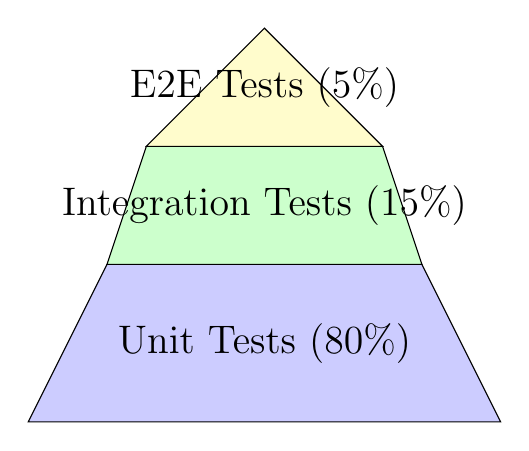
\begin{tikzpicture}
        \draw[fill=blue!20] (0,0) -- (6,0) -- (5,2) -- (1,2) -- cycle;
        \draw[fill=green!20] (1,2) -- (5,2) -- (4.5,3.5) -- (1.5,3.5) -- cycle;
        \draw[fill=yellow!20] (1.5,3.5) -- (4.5,3.5) -- (3,5) -- (3,5) -- cycle;
        
        \node at (3,1) {\Large Unit Tests (80\%)};
        \node at (3,2.75) {\Large Integration Tests (15\%)};
        \node at (3,4.25) {\Large E2E Tests (5\%)};
    \end{tikzpicture}
    \caption{Testing Pyramid Strategy}
    \label{fig:test-pyramid}
\end{figure}

\section{Unit Testing}

\textbf{Framework:} pytest

\textbf{Coverage Target:} 70\%+

\begin{lstlisting}[style=pythonstyle, caption={Unit Test Example}]
def test_trip_request_validation():
    # Valid request
    request = TripRequest(
        destination="Paris",
        start_date="2026-06-15",
        end_date="2026-06-18",
        budget=1500,
        travelers=2,
        interests=["culture"],
        pace="balanced"
    )
    assert request.destination == "Paris"
    
    # Invalid date
    with pytest.raises(ValidationError):
        TripRequest(
            destination="Paris",
            start_date="2026-06-18",
            end_date="2026-06-15",  # Before start_date
            budget=1500,
            travelers=2,
            interests=["culture"],
            pace="balanced"
        )
\end{lstlisting}

\section{Integration Testing}

\begin{lstlisting}[style=pythonstyle, caption={Integration Test Example}]
@pytest.mark.integration
@pytest.mark.asyncio
async def test_trip_planning_integration():
    request = TripRequest(
        destination="Paris, France",
        start_date="2026-06-15",
        end_date="2026-06-18",
        budget=1500,
        travelers=2,
        interests=["culture", "food"],
        pace="balanced"
    )
    
    service = TripService()
    response = await service.plan_trip(request)
    
    assert response.overview.destination == "Paris"
    assert len(response.itinerary) == 4
    assert response.smart_additions.packing_list
\end{lstlisting}

\section{API Testing}

\begin{lstlisting}[style=pythonstyle, caption={API Test Example}]
from fastapi.testclient import TestClient

client = TestClient(app)

def test_health_endpoint():
    response = client.get("/api/health")
    assert response.status_code == 200
    assert response.json()["status"] == "healthy"

def test_plan_trip_endpoint():
    request_data = {
        "destination": "Paris, France",
        "start_date": "2026-06-15",
        "end_date": "2026-06-18",
        "budget": 1500,
        "travelers": 2,
        "interests": ["culture", "food"],
        "pace": "balanced"
    }
    
    response = client.post("/api/plan-trip", json=request_data)
    assert response.status_code == 200
    data = response.json()
    assert "overview" in data
    assert "itinerary" in data
\end{lstlisting}

\section{Performance Testing}

\begin{lstlisting}[style=pythonstyle, caption={Load Test with Locust}]
from locust import HttpUser, task, between

class TripPlannerUser(HttpUser):
    wait_time = between(1, 5)
    
    @task
    def plan_trip(self):
        self.client.post("/api/plan-trip", json={
            "destination": "Paris, France",
            "start_date": "2026-06-15",
            "end_date": "2026-06-18",
            "budget": 1500,
            "travelers": 2,
            "interests": ["culture", "food"],
            "pace": "balanced"
        })
\end{lstlisting}

\textbf{Performance Criteria:}
\begin{itemize}
    \item 95th percentile response time $<$ 60s
    \item Support 10 concurrent users
    \item Error rate $<$ 1\%
    \item Memory usage $<$ 500MB per worker
\end{itemize}

%========================================
% CHAPTER 13: APPENDICES
%========================================
\chapter{Appendices}

\section{PlantUML Diagram Codes}

All PlantUML diagram codes are provided in separate files for easy copying and rendering.

\textbf{Available Diagram Files:}
\begin{enumerate}
    \item \texttt{diagrams/system-context-diagram.puml}
    \item \texttt{diagrams/high-level-architecture-diagram.puml}
    \item \texttt{diagrams/component-architecture-diagram.puml}
    \item \texttt{diagrams/data-flow-diagram.puml}
    \item \texttt{diagrams/deployment-architecture-diagram.puml}
    \item \texttt{diagrams/security-architecture-diagram.puml}
    \item \texttt{diagrams/ui-wireframe.puml}
    \item \texttt{diagrams/er-diagram-future.puml}
    \item \texttt{sequence-diagram.puml} (existing)
    \item \texttt{data-models-diagram.puml} (existing)
\end{enumerate}

\textbf{Rendering Instructions:}

See \texttt{DIAGRAMS-APPENDIX.md} for complete PlantUML codes and rendering instructions for all diagrams.

\section{Technology Stack Summary}

\begin{table}[H]
\centering
\small
\begin{tabular}{|l|l|p{6cm}|}
\hline
\textbf{Layer} & \textbf{Technology} & \textbf{Purpose} \\
\hline
Frontend & HTML5, CSS3, JavaScript & User interface \\
\hline
Backend Framework & FastAPI 0.100+ & REST API server \\
\hline
AI Framework & LangChain 0.1+ & Agent orchestration \\
\hline
LLM Provider & Groq API & AI inference \\
\hline
LLM Model & Llama 3.1 8B Instant & Fast language model \\
\hline
Validation & Pydantic 2.0+ & Data validation \\
\hline
HTTP Client & httpx & Async HTTP requests \\
\hline
ASGI Server & Uvicorn & Production server \\
\hline
Geocoding & OSM Nominatim & Location coordinates \\
\hline
Weather & Open-Meteo & Weather forecasts \\
\hline
POI & Overpass API & Points of interest \\
\hline
Routing & OpenRouteService & Route calculation \\
\hline
Containerization & Docker & Deployment \\
\hline
Testing & pytest & Unit/integration tests \\
\hline
\end{tabular}
\caption{Complete Technology Stack}
\label{tab:tech-stack}
\end{table}

\section{API Endpoint Summary}

\begin{table}[H]
\centering
\begin{tabular}{|l|l|p{6cm}|l|}
\hline
\textbf{Endpoint} & \textbf{Method} & \textbf{Purpose} & \textbf{Auth} \\
\hline
\texttt{/} & GET & API information & None \\
\hline
\texttt{/api/plan-trip} & POST & Generate itinerary & None \\
\hline
\texttt{/api/health} & GET & Health check & None \\
\hline
\texttt{/api/sample-request} & GET & Example request & None \\
\hline
\texttt{/docs} & GET & Swagger UI & None \\
\hline
\texttt{/redoc} & GET & ReDoc UI & None \\
\hline
\end{tabular}
\caption{Complete API Endpoint List}
\label{tab:api-endpoints-full}
\end{table}

\section{Configuration Variables}

\begin{table}[H]
\centering
\small
\begin{tabular}{|l|l|l|p{5cm}|}
\hline
\textbf{Variable} & \textbf{Required} & \textbf{Default} & \textbf{Description} \\
\hline
\texttt{GROQ\_API\_KEY} & Yes & - & Groq API authentication \\
\hline
\texttt{OPENROUTE\_API\_KEY} & No & - & OpenRouteService (optional) \\
\hline
\texttt{HOST} & No & 0.0.0.0 & Server bind address \\
\hline
\texttt{PORT} & No & 8000 & Server port \\
\hline
\texttt{DEBUG} & No & True & Debug mode \\
\hline
\texttt{CORS\_ORIGINS} & No & localhost & Allowed origins \\
\hline
\end{tabular}
\caption{Environment Configuration Variables}
\label{tab:config-vars}
\end{table}

\section{Error Code Reference}

\begin{table}[H]
\centering
\small
\begin{tabular}{|l|c|p{5cm}|p{4cm}|}
\hline
\textbf{Code} & \textbf{HTTP} & \textbf{Description} & \textbf{User Action} \\
\hline
\texttt{INVALID\_DATE} & 400 & Invalid date format/logic & Check date inputs \\
\hline
\texttt{INVALID\_BUDGET} & 400 & Budget too low & Increase budget \\
\hline
\texttt{LOCATION\_NOT\_FOUND} & 400 & Destination not found & Check spelling \\
\hline
\texttt{VALIDATION\_ERROR} & 422 & Pydantic validation failed & Fix input data \\
\hline
\texttt{API\_KEY\_MISSING} & 500 & Groq API key not set & Contact admin \\
\hline
\texttt{EXTERNAL\_API\_ERROR} & 503 & External service unavailable & Retry later \\
\hline
\texttt{LLM\_ERROR} & 500 & LLM failed to generate & Retry request \\
\hline
\texttt{RATE\_LIMIT\_EXCEEDED} & 429 & Too many requests & Wait and retry \\
\hline
\end{tabular}
\caption{Error Code Reference}
\label{tab:error-codes}
\end{table}

\section{Glossary}

See Table \ref{tab:definitions} on page \pageref{tab:definitions} for complete definitions and acronyms.

\section{Change Log}

\begin{table}[H]
\centering
\begin{tabular}{|c|c|p{7cm}|p{3cm}|}
\hline
\textbf{Version} & \textbf{Date} & \textbf{Changes} & \textbf{Author} \\
\hline
1.0 & 2026-02-25 & Initial design document & Development Team \\
\hline
\end{tabular}
\caption{Document Change Log}
\label{tab:changelog}
\end{table}

%========================================
% DOCUMENT APPROVAL
%========================================
\chapter*{Document Approval}
\addcontentsline{toc}{chapter}{Document Approval}

\begin{table}[H]
\centering
\begin{tabular}{|l|p{4cm}|p{4cm}|p{3cm}|}
\hline
\textbf{Role} & \textbf{Name} & \textbf{Signature} & \textbf{Date} \\
\hline
Lead Architect & & & \\[0.8cm]
\hline
Backend Lead & & & \\[0.8cm]
\hline
Frontend Lead & & & \\[0.8cm]
\hline
DevOps Lead & & & \\[0.8cm]
\hline
QA Lead & & & \\[0.8cm]
\hline
Technical Director & & & \\[0.8cm]
\hline
\end{tabular}
\caption*{Approval Signatures}
\end{table}

\vspace{2cm}

\begin{center}
\textbf{--- End of Design Document ---}

\vspace{1cm}

\textit{This document is subject to change. All updates should be reviewed and approved by the technical leads.}
\end{center}

\end{document}
